\chapter{Neurónové siete} \label{cha:neural-networks}

Táto kapitola popisuje obecne princíp neurónových sietí, ktoré využijeme v~našej práci na viacero úloh -- odhad pravdepodobností v~akustickom modeli, odhad fonologických rysov, a taktiež na klasifikáciu výslovnosti. Informácie v~tejto kapitole sú primárne založené na publikácii \cite{Bishop2006}. 

\section{Dopredné neurónové siete}

Neurónové siete sú dnes dominantnou metódou využívanou na strojové učenie, kde dosahujú výrazne lepšie výsledky ako iné konvenčné metódy. Neurónová sieť je biologicky inšpirovaný matematický model, ktorý mapuje vstupné vektory na zodpovedajúce výstupné vektory. Dimenzie týchto vektorov môžu byť obecne rôzne. 

Najrozšírenejším typom neurónovej siete je neurónová sieť s~dopredným šírením (\textit{feedforward neural network}), v~ktorej sa informácia šíri jedným smerom zo vstupu na výstup. To znamená, že v~nej neexistujú žiadne spätné väzby. 

Neuróny v~doprednej neurónovej sieti sa zvyčajne organizujú do vrstiev, kde prvá vrstva sa označuje ako vstupná, za ňou nasleduje skrytá vrstva a posledná vrstva je vrstvou výstupnou. Skrytých vrstiev môže sieť obsahovať niekoľko, kedy takéto siete zvykneme označovať ako hlboké neurónové siete (\textit{Deep Neural Network}, DNN), ale nie sú výnimkou ani siete bez skrytej vrstvy. Najčastejšie sú jednotlivé vrstvy medzi sebou plne prepojené, čo znamená, že všetky výstupy z~jednej vrstvy sú privedené na všetky vstupy tej nasledujúcej. Príklad neurónovej siete s~jednou skrytou vrstvou je možné vidieť na obrázku \ref{fig:nn}.

\begin{figure}[!ht]
    \centering
    \newif\ifstandalone
\standalonetrue % comment out for compilation with ktikz	

\ifstandalone
\documentclass{standalone}
\fi

\usetikzlibrary{shapes.geometric, arrows, positioning, arrows.meta, calc}

\ifstandalone
\begin{document}
\fi

\def\layersep{2.5cm}

\begin{tikzpicture}[shorten >=1pt,->,draw=black!50, node distance=\layersep]
    \tikzstyle{every pin edge}=[<-,shorten <=1pt]
    \tikzstyle{neuron}=[circle,fill=black!25,minimum size=17pt,inner sep=0pt]
    \tikzstyle{input neuron}=[neuron, fill=green!60];
    \tikzstyle{output neuron}=[neuron, fill=red!60];
    \tikzstyle{hidden neuron}=[neuron, fill=blue!60];
    \tikzstyle{annot} = [text width=4em, text centered]

    % Draw the input layer nodes
    \foreach \name / \y in {1,...,4}
    % This is the same as writing \foreach \name / \y in {1/1,2/2,3/3,4/4}
        \node[input neuron, pin=left:$x_\y$] (I-\name) at (0,-\y) {};

    % Draw the hidden layer nodes
    \foreach \name / \y in {1,...,5}
        \path[yshift=0.5cm]
			node[hidden neuron] (H-\name) at (\layersep,-\y cm) {};
			
	% Draw the hidden layer nodes
	\foreach \name / \y in {1,...,3}
       \path[yshift=-0.5cm]
            node[output neuron, pin={[pin edge={->}]right:$y_\y$}] (O-\name) at (2*\layersep,-\y cm) {};

    % Draw the output layer node
    % \node[output neuron,pin={[pin edge={->}]right:Výstup}, right of=H-2] (O) {};

    % Connect every node in the input layer with every node in the
    % hidden layer.
    \foreach \source in {1,...,4}
        \foreach \dest in {1,...,5}
			\path (I-\source) edge (H-\dest);

	% Connect every node in the hidden layer with every node in 
	% the output layer
	\foreach \source in {1,...,5}
	\foreach \dest in {1,...,3}
		\path (H-\source) edge (O-\dest);

    % \foreach \source in {0,...,4}
        % \path (H-\source) edge (O);

    % Annotate the layers
    \node[annot,above of=H-1, node distance=1cm] (hl) {Skrytá vrstva};
    \node[annot,left of=hl] {Vstupná vrstva};
    \node[annot,right of=hl] {Výstupná vrstva};
\end{tikzpicture}

\ifstandalone
\end{document}
\fi
    \caption{Príklad neurónovej siete s~jednou skrytou vrstvou.}
    \label{fig:nn}
\end{figure}

Ako už bolo naznačené, základnou jednotkou neurónovej siete je neurón, ktorý transformuje vstupný vektor $x = (x_1, \dots, x_N)$ na hodnotu $y$ pomocou vzťahu

\begin{equation}
    y = f\left(\sum_{i=1}^N{w_i x_i} + b\right),
\end{equation}

\noindent kde $w = (w_1, \dots, w_N)$ predstavuje vektor váh, $b$ prahovú hodnotu, a $f$ je nejaká vhodne zvolená funcia. Ak rozšírime vstupný vektor $x$ o~hodnotu $x_0 = 1$, môžeme prahovú hodnotu $b$ zakomponovať do vektoru $w$, čiže $w_0 = b$. Potom môžeme vyššie uvedený vzťah upraviť na

\begin{equation}
    y = f\left(\sum_{i=0}^N{w_i x_i}\right).
\end{equation}

\noindent Podstatnou časťou, ktorá má vplyv na správne fungovanie neurónovej siete, je funkcia $f(.)$, zväčša označovaná ako aktivačná funkcia. Aby bola neurónová sieť schopná realizovať nelineárne mapovanie vstupov na výstup, musí byť aj táto funkcia nelineárna. Okrem toho k~nej musí existovať derivácia, aby bolo možné trénovanie s~využitím spätného šírenia chyby. Vhodnými funkciami sú napr. logistická sigmoida, hyperbolický tangens alebo ReLU, viď tabuľku \ref{tab:activation-functions}. Posledná menovaná je vhodná najmä pre použitie v~skrytých vrstvách DNN, nakoľko umožňuje lepšie propagovanie gradientov pri trénovaní \cite{Glorot2011}. V~prípade použitia neurónovej siete na klasifikáciu sa pri výstupnej vrstve využíva výhradne logistická sigmoida alebo softmax funkcia. Výstupom oboch funkcií sú hodnoty od 0 do 1, ktoré je možné interpretovať ako pravdepodobnosti. Softmax funkcia naviac realizuje normalizáciu cez všetky neuróny danej vrstvy, vďaka čomu je suma výstupných hodnôt rovná 1. To sa hodí najmä pri klasifikácii 1 z~N, kedy potrebujeme, aby výstupy reprezentovali príslušnosť do nejakej triedy. 

\begin{table}[ht!]
    \centering
    \begingroup
    % \renewcommand{\arraystretch}{5.0}
    \begin{tabular}{@{}lll@{}}
    \toprule
    Názov                & Funkcia & Derivácia\\ \midrule
    Logistická sigmoida  & $\displaystyle f(x) = \frac{1}{1+e^{-x}}$ &  $\displaystyle f'(x) = f(x)(1-f(x))$    \\
    Hyperbolický tangens & \rule{0pt}{0.8cm}$\displaystyle f(x) = \frac{e^x - e^{-x}}{e^x - e^{-x}}$  & $\displaystyle f'(x) = 1 - f(x)^2$   \\
    ReLU                 & \rule{0pt}{0.8cm}$\displaystyle f(x) = \begin{cases} 0 & x < 0 \\ x & x \geq 0 \end{cases}$  & $\displaystyle f'(x) = \begin{cases} 0 & x < 0 \\ 1 & x \geq 0 \end{cases}$   \\ \bottomrule
    \end{tabular}
    \endgroup
    \caption{Najčastejšie používané aktivačné funkcie a ich derivácie.} \label{tab:activation-functions}
\end{table}

\subsection*{Trénovanie}

Cieľom trénovania je nájdenie vhodných parametrov $w$ u~jednotlivých neurónov. K~tomu sa používa tzv. iteratívne trénovanie s~učiteľom, kedy sa v~každej iterácii vypočíta chyba medzi predikciami neurónovej siete a známym výstupom. Na základe tejto chyby sa potom upravia váhy jednotlivých neurónov. Najčastejšie sa k~tomu používa algoritmus \textit{stochastic gradient-descent} v~kombinácii so spätnou propagáciou chyby, ktorý aktualizuje váhy neurónov v~jednotlivých vrstvách výpočtom gradientov chybovej funkcie. 

Dôležitá je aj voľba samotnej chybovej funkcie. Najpoužívanejšími sú stredná kvadratická chyba, krížová entropia a kategorická krížová entropia. Posledné dve menované sú vhodné pre klasifikačné úlohy, pričom kategorická krížová entropia sa využíva výhradne v~kombinácii so softmax výstupnou vrstvou.

V~tejto sekcii sme uviedli len základný popis dopredných neurónových sietí a ich fungovania. Pre ďalšie podrobnosti viď \cite{Bishop2006}.

\section{Rekurentné neurónové siete} 

Rekurentné neurónové siete (\textit{Recurent Neural Networks}, RNN) narozdiel od dopredných sietí umožňujú zavádzanie spätných väzieb. To spôsobí, že aktuálny výstup siete nie je závislý len na aktuálnom vstupe, ale aj na vstupoch predcházajúcich. RNN teda umožujú zachytiť časové závislosti medzi dátami, ktoré sú dôležité pre mnoho úloh, ako je aj spracovanie reči.

Obrázok \ref{fig:RNN-diagram} znázorňuje jednoduchú RNN pozostávajúcu z~jedinej vrstvy $H$. Na jej vstup je okrem aktuálneho vzorku $x_t$ privedený aj predchádzajúci výstup $h_{t-1}$ odpovedajúci vzorke $x_{t-1}$. Na takúto sieť môžeme nazerať ako na niekoľko kópii tej istej siete, ktoré predávajú svoje výstupy svojim následovníkom, tak ako je to znázornené na obr. \ref{fig:RNN-diagram}.

\begin{figure}[ht!]
    \centering
    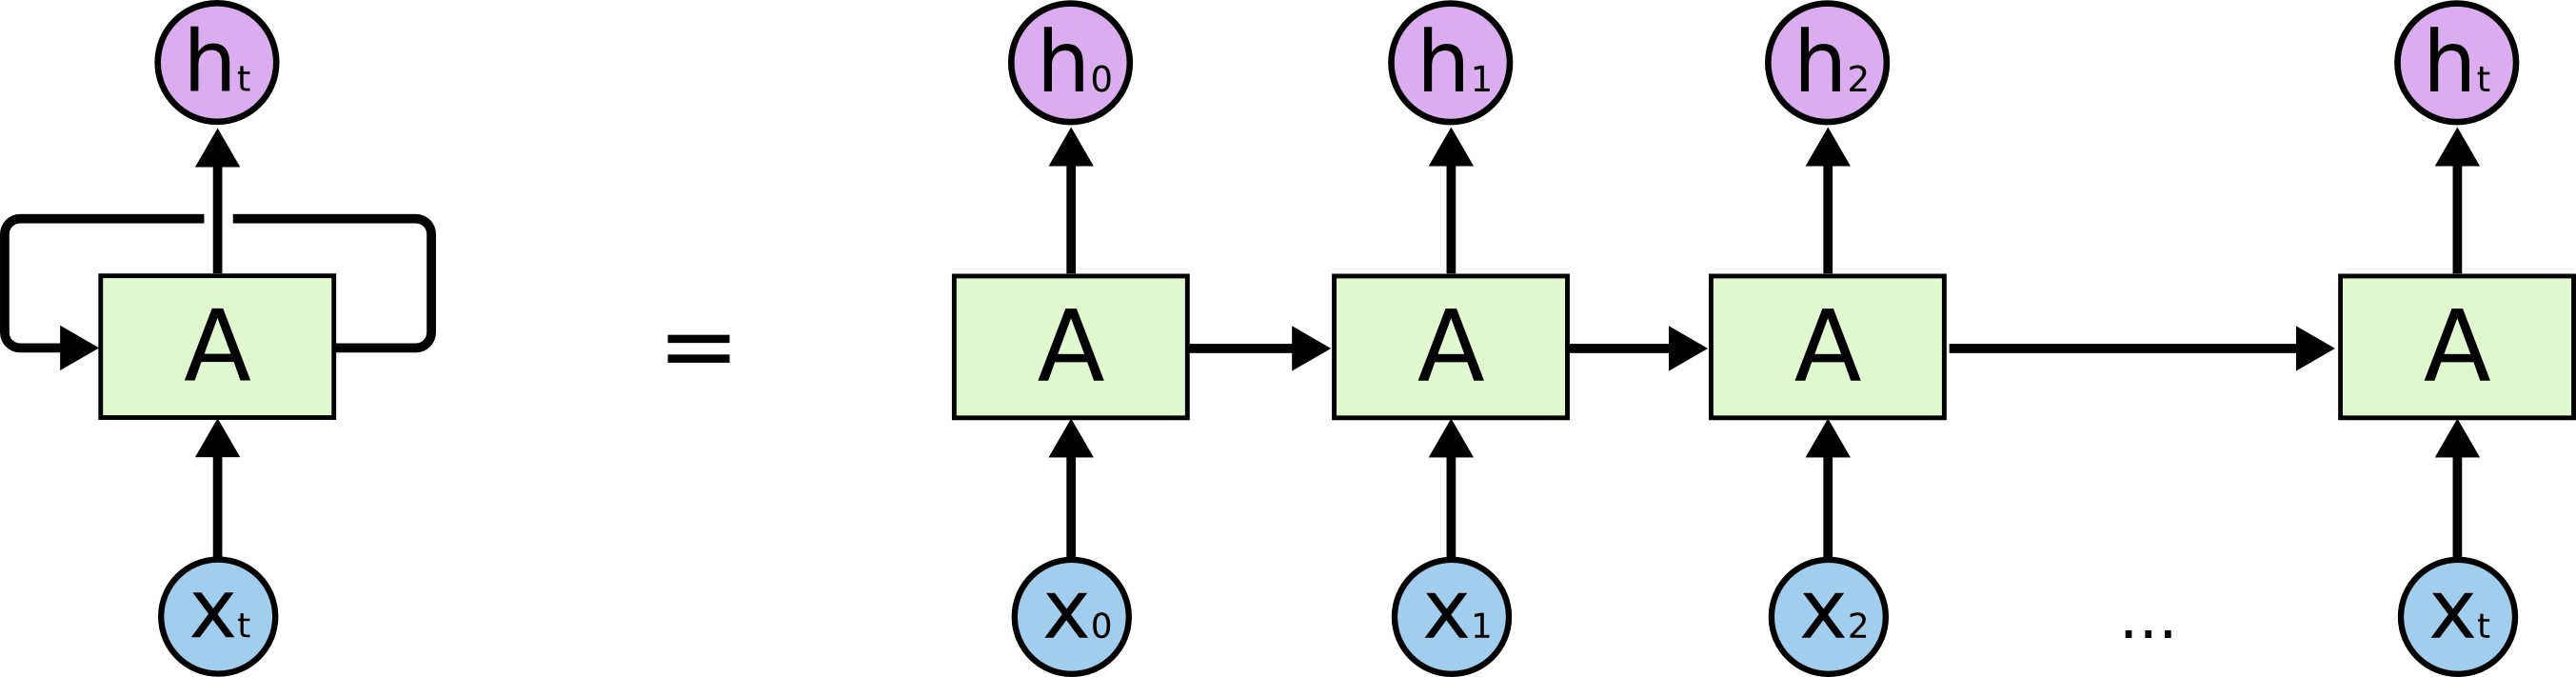
\includegraphics[width=.8\textwidth]{figures/RNN-unrolled.png}
    \caption{Schéma základnej RNN s~jednou skrytou vrstvou. Vľavo je znázornená spätná väzba pomocou cyklu, vpravo rozbalená sieť pre jednotlivé vstupné vzorky $x_0, \dots, x_t$. Prevzaté z~\cite{Olah2015}.}
    \label{fig:RNN-diagram}
\end{figure}

\noindent Siete s~takouto architektúrou však majú v~praxi problém zachytiť závislosti medzi vzorkami vzdiaľenými ďaleko od seba. Preto sa v~súčasnosti používajú špeciálny typ RNN, tzv. \textit{Long short-term memory} (LSTM) siete, u~ktorých tento problém nie je tak výrazný.

\subsection*{LSTM neurónové siete}

LSTM neurónové siete nie sú organizované do vrstiev, ako tomu bolo doteraz, ale sú tvorené komplexnými jednotkami realizujúcimi viacero operácii nad vstupnými dátami. Porovnanie jednoduchej RNN a LSTM je možné vidieť na obrázku \ref{fig:RNN-vs-LSTM}. Zatiaľ čo RNN tvorí zväčša jediná vrstva, v~tomto prípade s~aktivačnou funkciou hyperbolický tangens, LSTM jednotka pozostáva z~niekoľkých vrstiev s~aktivačnými funkciami logistická sigmoida a hyperbolický tangens. Výstupy týchto vrstiev sú následne kombinované operáciami násobenia a sčítania, čím produkujú dva výstupy $h_t$ a $C_t$. Druhý menovaný výstup slúži len na predanie pomocnej informácie do ďalšieho kroku výpočtu, viď obr. \ref{fig:LSTM-chain}. Vďaka tejto dodatočnej komunikačnej linke sú jednotky schopné pridať váhu dôležitým vstupným vzorkám v~sekvencii, a naopak potlačiť menej významné vzorky. Pre detailnejší popis fungovania LSTM sietí odporúčame článok \cite{Olah2015}.

\begin{figure}[ht!]
    \centering
    \begin{subfigure}{.49\textwidth}
        \centering
        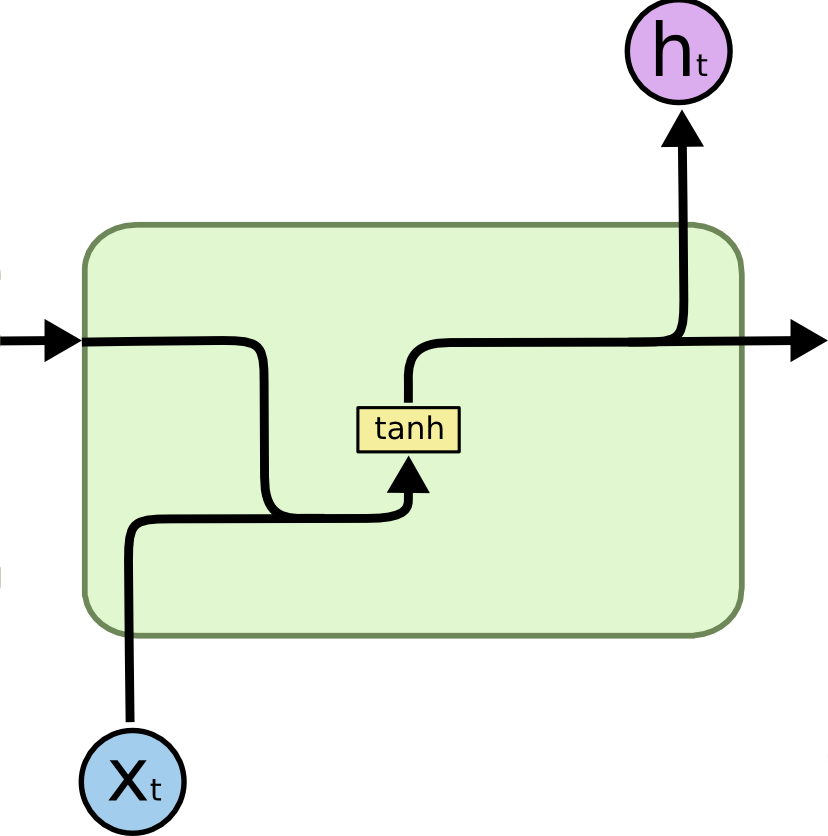
\includegraphics[width=0.7\linewidth]{figures/SimpleRNN-unit.png}   
        \caption{RNN}
        \label{fig:SimpleRNN-unit}
    \end{subfigure}
    \begin{subfigure}{.49\textwidth}
        \centering
        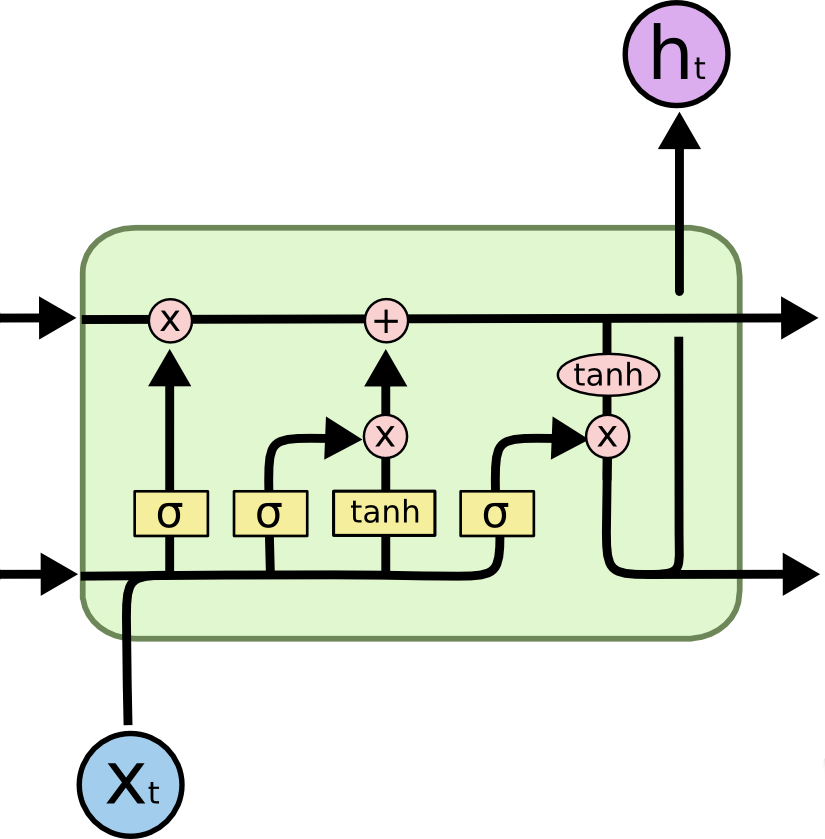
\includegraphics[width=0.7\linewidth]{figures/LSTM-unit.png}   
        \caption{LSTM}
        \label{fig:LSTM-unit}
    \end{subfigure}
    \caption{Porovnanie architektúry jednoduchej RNN a LSTM neurónovej siete. Prevzaté z~\cite{Olah2015}.} \label{fig:RNN-vs-LSTM}
\end{figure}

\begin{figure}[ht!]
    \centering
    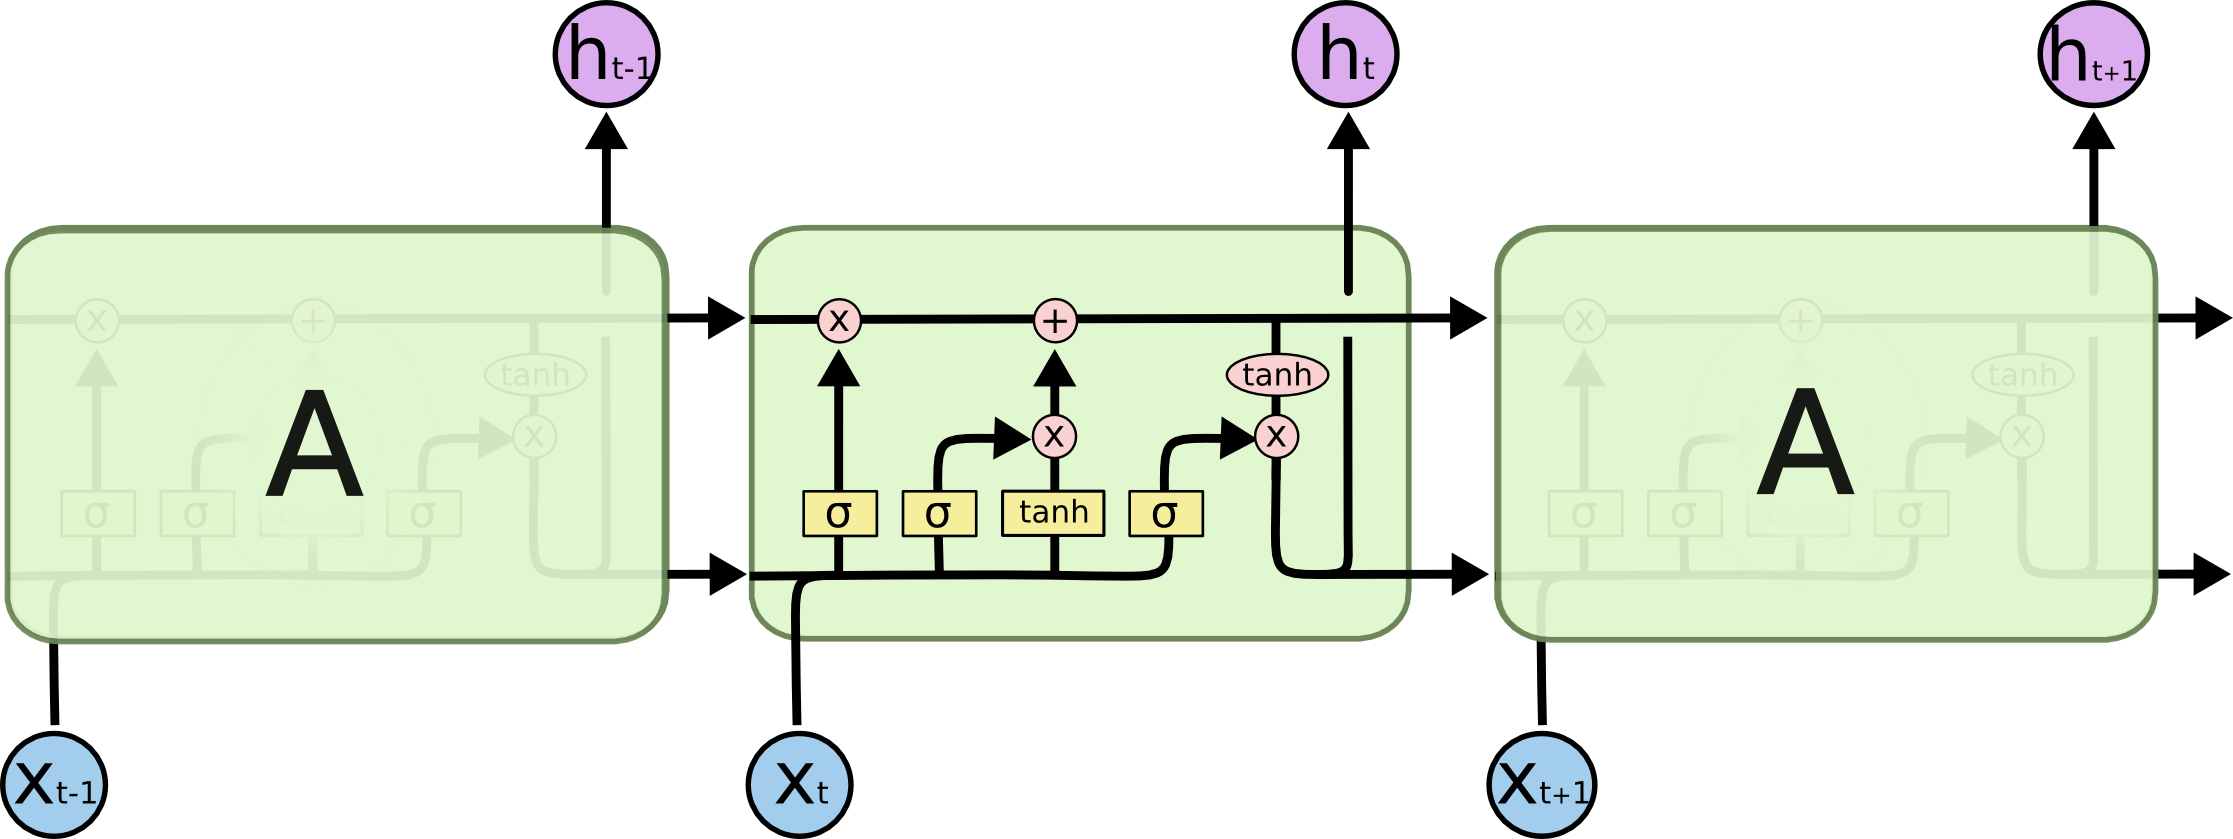
\includegraphics[width=0.8\textwidth]{figures/LSTM-chain.png}
    \caption{Znázornenie spätných väzieb pri LSTM jednotkách spracovávajúcich vzorky $x_{t-1}, x_t, x_{t+1}$. Prevzaté z~\cite{Olah2015}.}
    \label{fig:LSTM-chain}
\end{figure}

\section{Použitie neurónových sietí k~rozpoznávaniu reči}

V~súčasnosti bývajú neurónové siete čoraz častejšie využívané v~systémoch rozpoznávania reči. Zväčša bývajú použité na realizáciu tzv. DNN-HMM akustických modelov, kde DNN nahrádza v~minulosti často používané modely zmesí normálnych rozložení v~GMM-HMM akustických modeloch. 

Ako už bolo spomenuté, pri akustickom modeli potrebujeme určiť pre rámce reči $\bm{o}_t$ výstupné pravdepodobnosti $b_j(\bm{o}_t)$ pre jednotlivé HMM stavy $s_j$. Avšak aby sme k~tomuto účelu mohli natrénovať neurónovú sieť, musíme najskôr získať zarovnanie reči na jednotlivé stavy $s_j$. K~tomuto účelu sa využíva vopred natrénovaný GMM-HMM model.

Na vstup DNN sa privádzajú príznaky zodpovedajúce rámcu $\bm{o}_t$. Keďže sa jedná o~klasifikáciu 1 z~N, výstupná DNN vrstva je tvorená softmax aktivačnou funkciou. Takto natrénovaná sieť potom určuje aposteriórne pravdepodobnosti $p(s_j|\bm{o}_t)$ stavov $s_j$. Takto získaná pravdepodobnosť však obsahuje aj informáciu o~apriórnej pravdepodobnosti stavov $P(s_j)$, ktorá je nadbytočná, nakoľko túto informáciu v~inej podobe a lepšie modeluje jazykový model. Preto je na záver ešte získané aposteriórne pravdepodobnosti $p(s_j|\bm{o}_t)$ potrebné previesť na vierodnosti, čo je možné pomocou vzťahu

\begin{equation}
    p(\bm{o}_t|s_j) = \frac{p(s_j|\bm{o}_t)}{P(s_j)} p(\bm{o}_t),
\end{equation}

\noindent kde $P(s_j)$ reprezentuje apriórne pravdepodobnosti $P(s_j)$, ktoré sa stanovia frekvenčnou analýzou. Čo ale nedokážeme určiť, je apriórna pravdepodobnosť príznakov rámca $p(\bm{o}_t)$. Našťastie to však ani nie je potrebné, nakoľko nie je závislá na stave $s_j$, takže ju je možné zo vzťahu úplne vypustiť, čím dostaneme

\begin{equation}
    p(\bm{o}_t|s_j) = \frac{p(s_j|\bm{o}_t)}{P(s_j)}.
\end{equation}